\chapter{Data Acquisition and Trigger}

\section{Counting House}

This section discusses the location and function of equipment located in the
Hall~C counting house, including fast electronics, computers, cabling,
terminals, etc.
Operating procedures are available for various subsystems, such as how to
run the data acquisition software.

\subsection{Cabling and Electronics}

The features of the data acquisition
electronics from the output of PMT's, through trigger and inputs, to
the Fastbus modules, are discussed in this section.
The philosophy of the Hall~C fast electronics is to bring all the
raw phototube signals into the counting house where the trigger and
digitization are. The only exceptions to this are the TDC's for all of
the wire chambers. Since the wire chambers use multi-hit TDC's in a
common stop mode, the common signal may arrive at the TDC modules long
after the individual inputs.

The readout electronics for all Hall~C detector systems (except the
drift chambers) are located in Counting House C (Bldg 97, room 101A).
There are seven primary racks in this counting house (Figure~\ref{fig:7.1}). 
\begin{figure}
%\htmlimage{thumbnail=0.5,flip=r270}
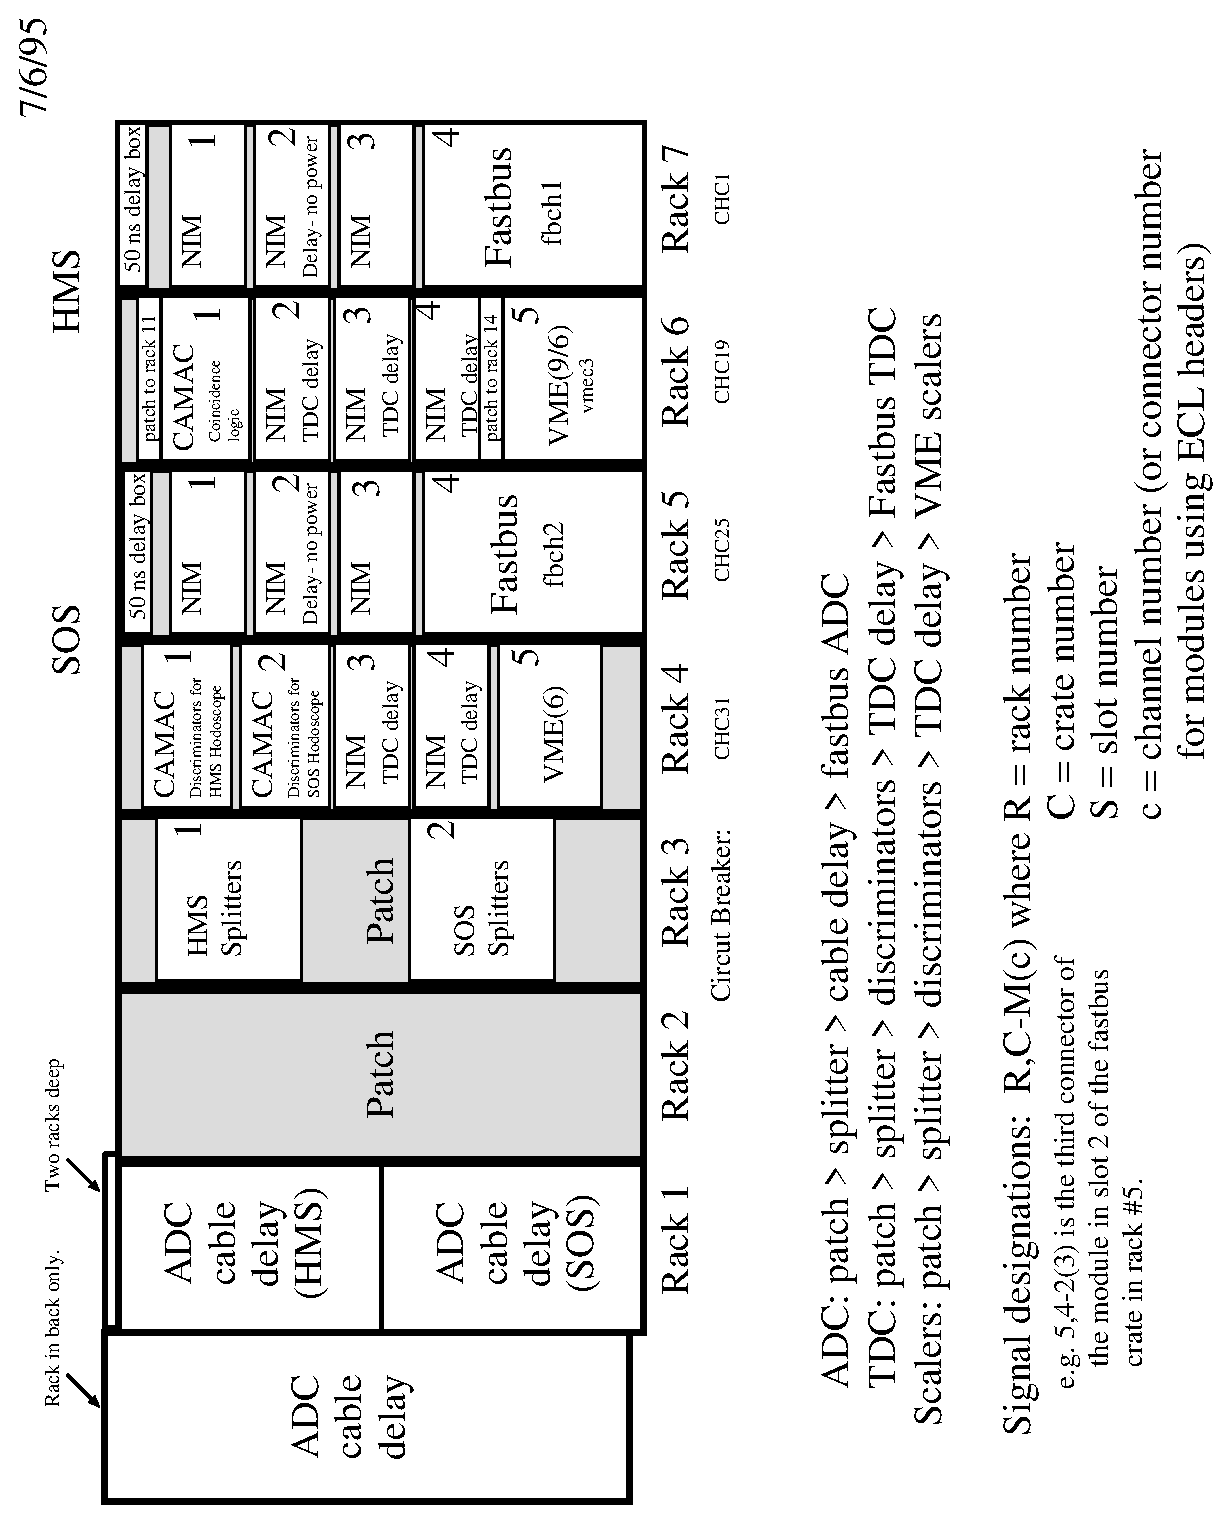
\includegraphics[width=6in]{daq_trig/racks.eps}
\caption{The Primary Racks in the Counting House\label{fig:7.1}}
\end{figure}
Two of these
contain the patch panels where the signals from the hall are
brought to the counting
house. The others contain the fast electronics used to form the trigger and to
readout the data. There are additional racks in the counting house
which contain electronics
related to the beam current monitors and beam rastering system. Figures~\ref{fig:7.2}-
\ref{fig:ts_logic} show the trigger electronics, arranged by detector system. Figure~\ref{fig:hms_trig_logic} depicts
the layout of the HMS trigger electronics.

\begin{figure}
%\htmlimage{thumbnail=0.5,flip=r270}
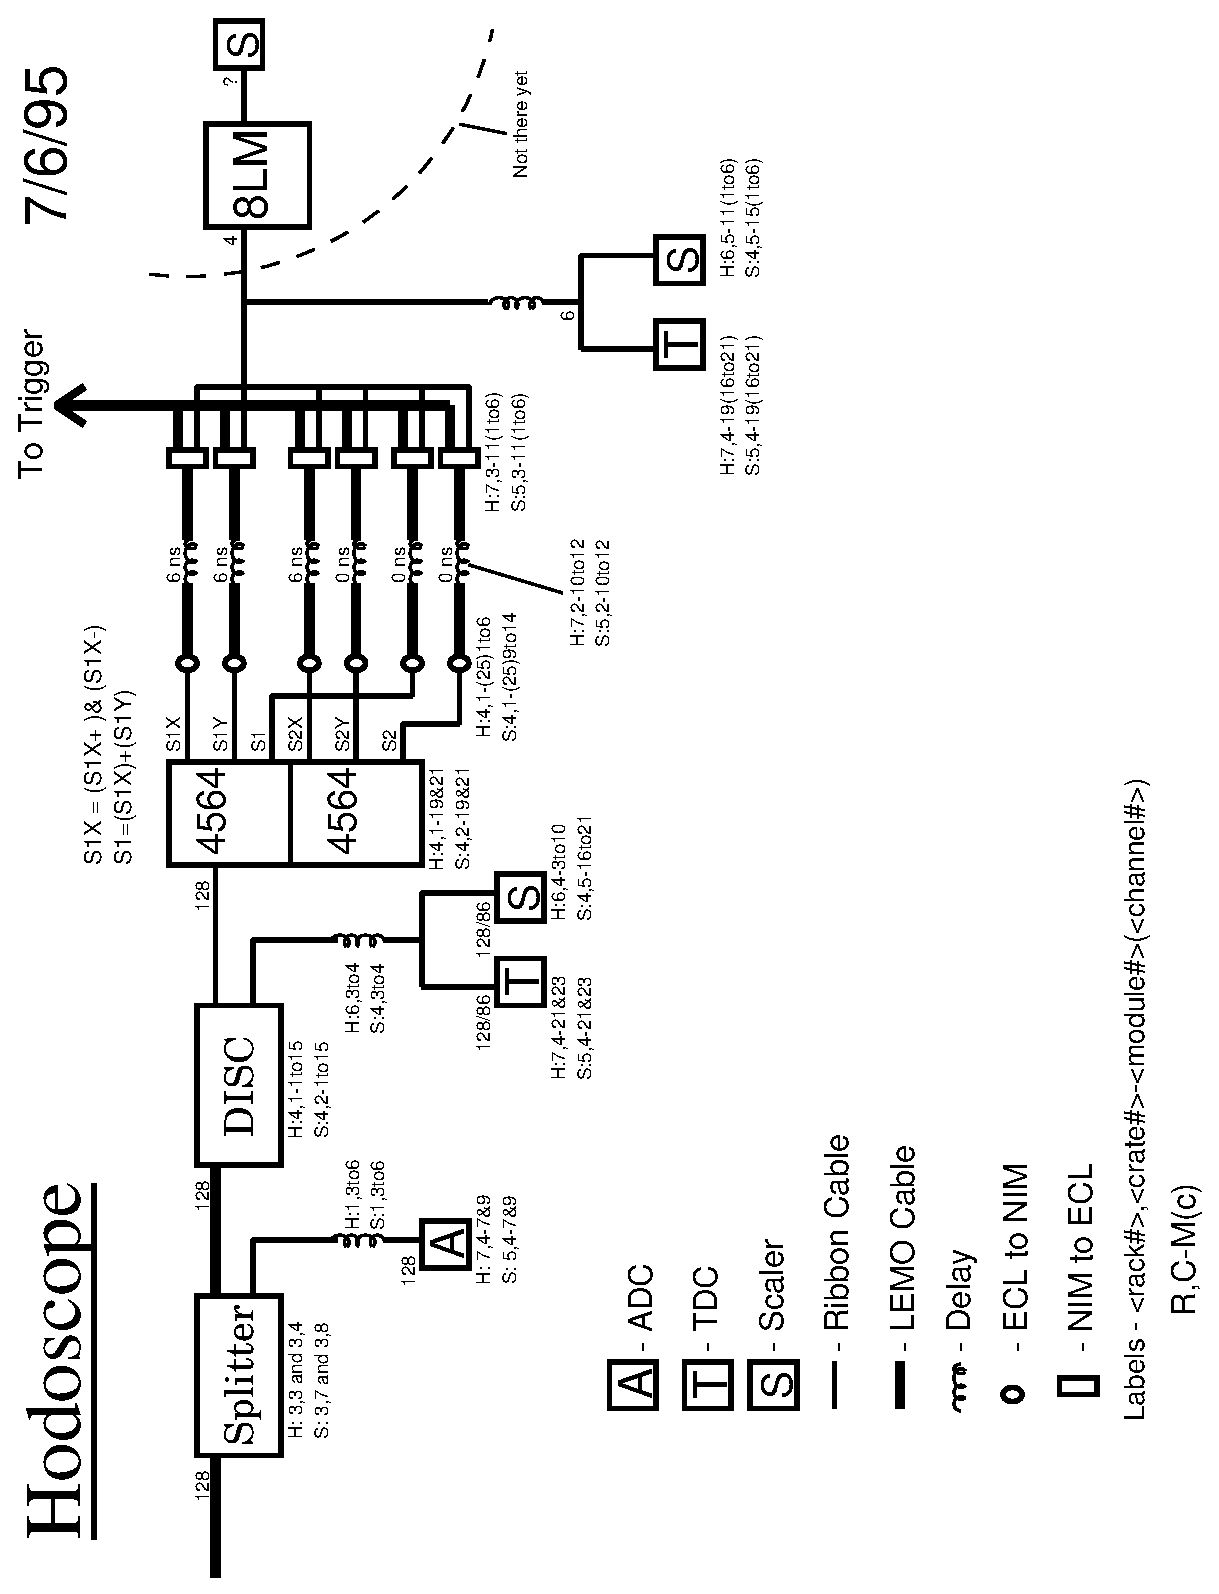
\includegraphics[width=5.8in]{daq_trig/hodoscope.eps}
\caption{Hall~C Fast Electronics (1 of 5) \label{fig:7.2}}
\end{figure}
\clearpage

\begin{figure}
%\htmlimage{thumbnail=0.5,flip=r270}
\includegraphics[width=5.8in,height=7in]{daq_trig/cerenkov.eps}
\caption{Hall~C Fast Electronics (2 of 5) \label{fig:7.3}}
\end{figure}
\clearpage

\begin{figure}
%\htmlimage{thumbnail=0.5,flip=r270}
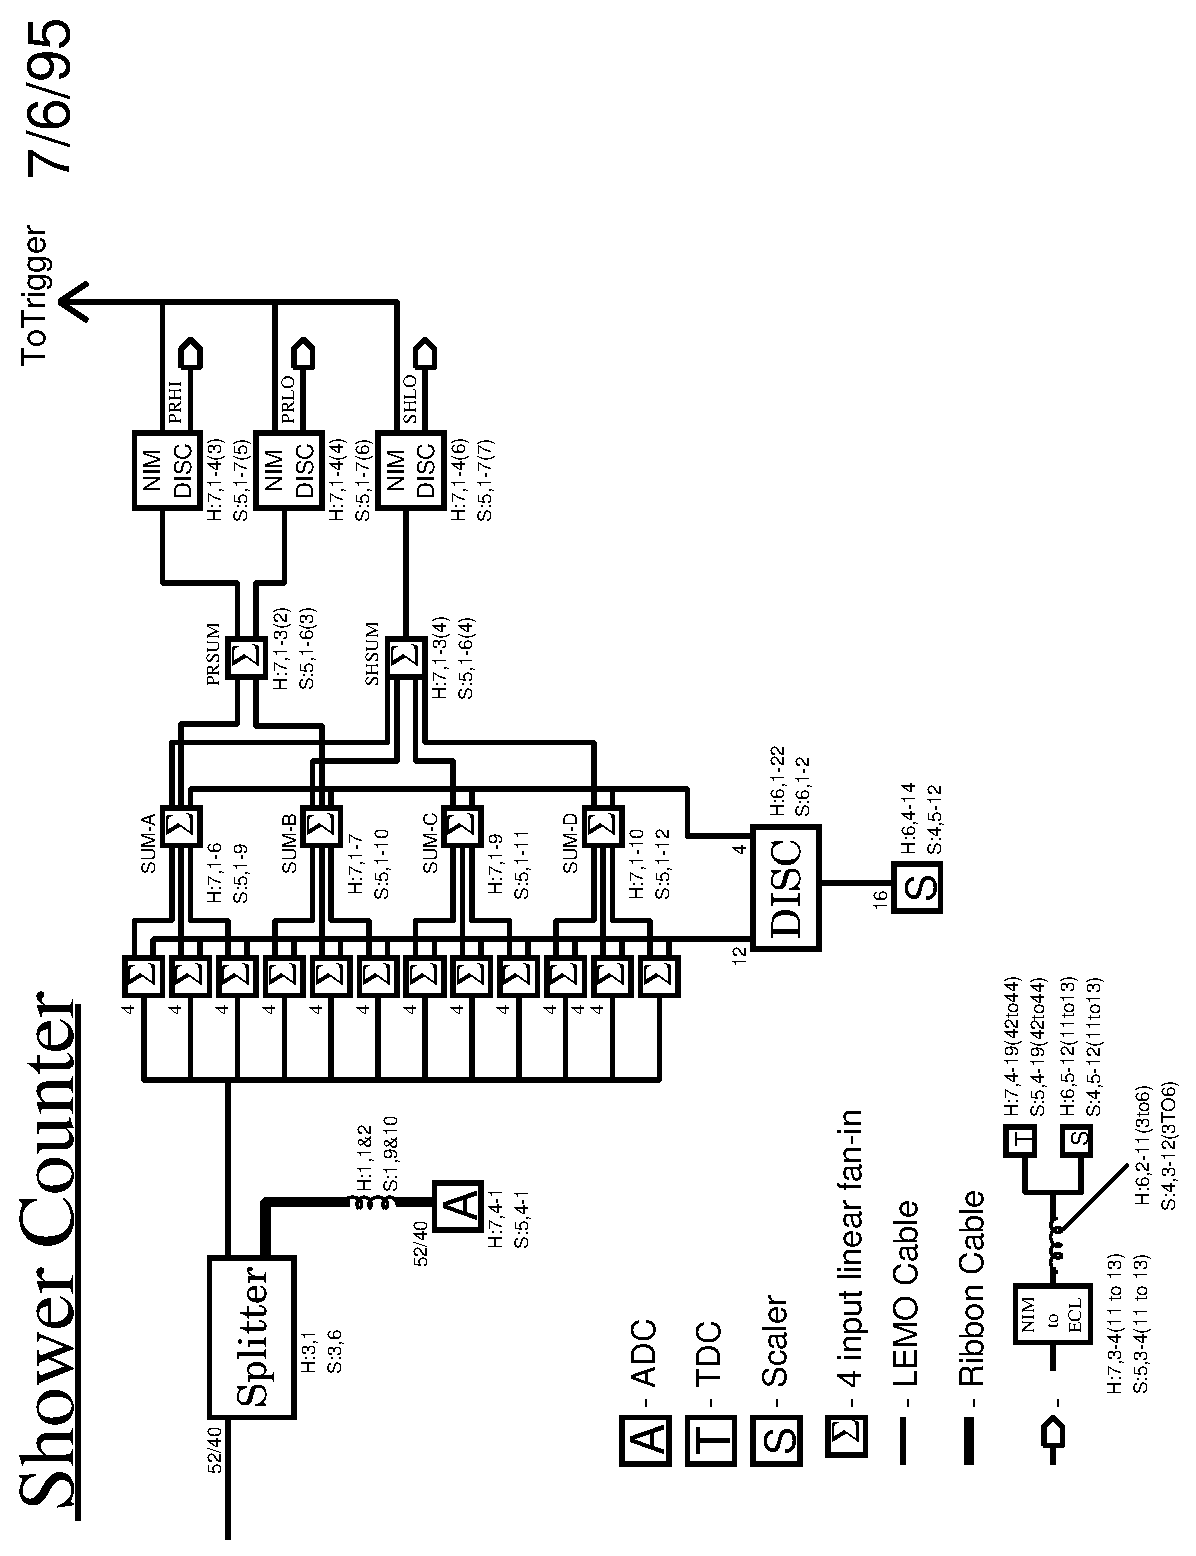
\includegraphics[width=5.8in]{daq_trig/shower.eps}
\caption{Hall~C Fast Electronics (3 of 5) \label{fig:shwr_logic}}
\end{figure}
\clearpage

\begin{figure}
%\htmlimage{thumbnail=0.5,flip=r270}
\includegraphics[width=5.8in,height=7in]{daq_trig/trig_9901.eps}
\caption{Hall~C Fast Electronics (4 of 5) \label{fig:trigger}}
\end{figure}
\clearpage

\begin{figure}
%\htmlimage{thumbnail=0.5,flip=r270}
\includegraphics[width=5.8in,height=7in]{daq_trig/ts_jan99.eps}
\caption{Hall~C Fast Electronics (5 of 5) \label{fig:ts_logic}}
\end{figure}
\clearpage

\begin{figure}
%\htmlimage{thumbnail=0.5}
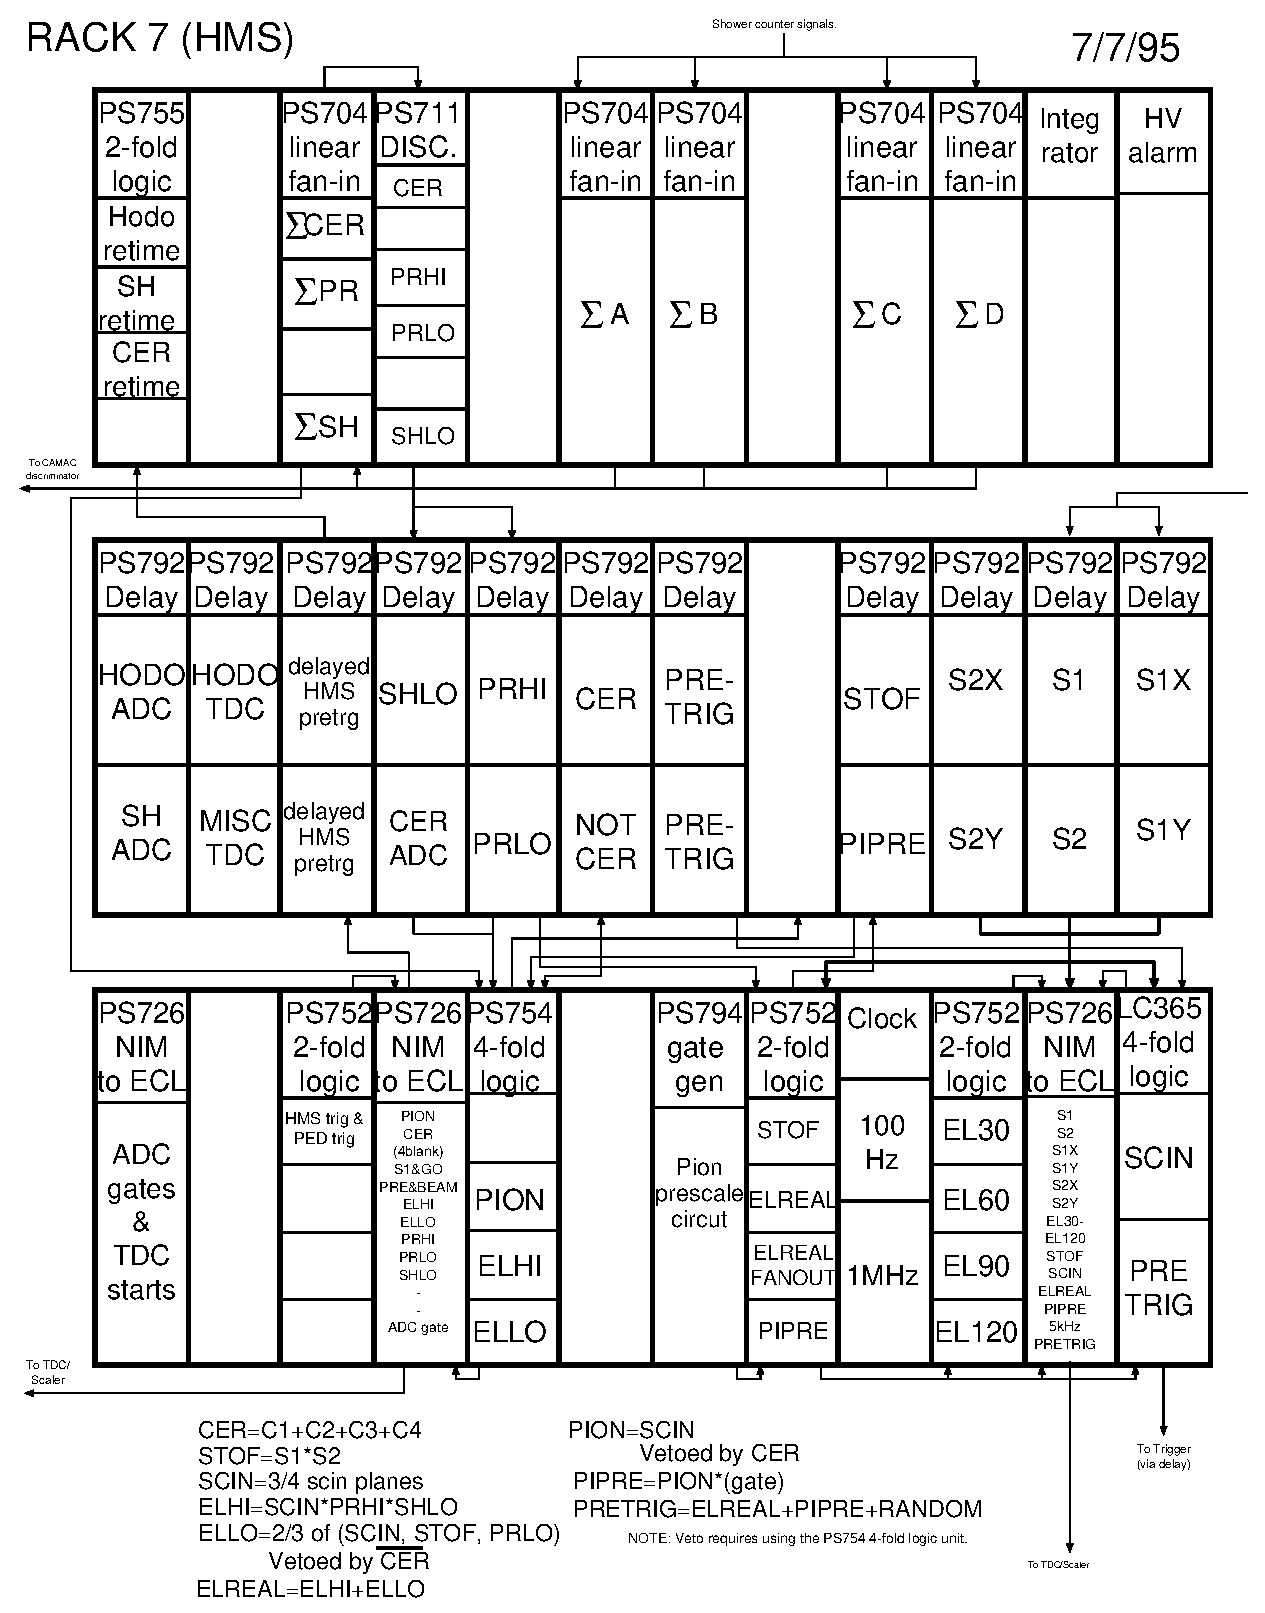
\includegraphics[width=5.8in]{daq_trig/hms_crates.eps}
\caption{HMS Trigger Electronics\label{fig:hms_trig_logic}}
\end{figure}
\clearpage

\subsubsection{Cabling}

The path that a signal follows from a PMT to the counting house is as
follows.
\begin{enumerate}
\item 30 ft length cables will run from the PMT's to a patch in the focal
plane hut.
\item 250(200) ft length cables run from the HMS(SOS) hut patch along the
spectrometer and through the pipes
under the floor to a patch near the personnel access to the hall.
\item 200 ft length cables run from the patch at the hall entrance
along the hallway wall and up the shaft.  They continue under the
computer floor and up to patches in the counting room.
\item 8 ft length LEMO cables run from the patch to the splitter (see
Figure~\ref{fig:7.1}).
\end{enumerate}
{(\bf Note: Cable lengths are unverified rough estimates.)}
The total length of the cable from the PMT's to the splitter is 560 ns.

Patch cable signal assignments are recorded in the document
\verb|~cdaq/documents/trigger/C_patches.txt|.

The cable runs for the SOS are similar except that an extra 100 ns worth
of cable has been added to the cable run before the splitter.  This extra length
of cable is located in the back of the SOS hut, just before the patch leading
from the hut to the floor of the hall. This  extra amount of cable is (with
great difficulty)
removable and the length has been chosen such that if a coincidence reaction
emits a $\beta = 1$ particle into each spectrometer, the signals will arrive
at the patch simultaneously.  The extra cable is removable to allow for
experiments with a very slow hadron in the SOS to be timed into a
coincidence with an electron in the HMS.

The splitters will make a possibly asymmetric split of the signal, one for the
discriminators, the other delayed for input into ADC's. UVA's design for a
compact splitter box handles 64 channels in 3 inches of 19 inch rack space,
with LEMO inputs which are split into LEMO outputs and into 34 pin headers.
The discriminators have two outputs per channel. One output will be used in
the trigger logic, the other channel will be delayed for input into high
resolution TDC's.

The types of delays for ADC and TDC inputs are :
\begin{itemize}
\item Delay with RG-8 or RG-58 feeding into a box that transfers the
signals to ribbon cable.
\item Digital delay boxes.
\end{itemize}
respectively. These delays are approximately 360 ns. The ADC is
the LeCroy 1881M Fastbus ADC using 34 pin headers for inputs.
The ADC's are configured to have an input termination of 50 ohm with a
fixed ground.

The input termination may be either 50 ohm with fixed ground,
50 ohm with floating ground, or  100 ohm pseudo-differential inputs.
They may also be used as single ended by grounding one pin.

% Not relevant
%The delay for the discriminator outputs must have time delay stability. If
%ribbon cable is used for the delay, we must keep the temperature of the
%cable stable. Dave Mack has found a temperature instability of XX ps per
%degree. We may want to boost the ECL signals just after the discriminator
%so that the signal inputs will still be large at the TDC inputs.

\subsubsection{Coincidence Electronics}

The trigger electronics has switchable 63.5 ns delays on the hodoscope
OR's for both spectrometers. This allows one spectrometer to be delayed
by up to 63.5 ns with respect to the other. For the purposes of computing
the range of velocities that can be brought into coincidence, these delays
shall be considered to have a range of at most $\pm$ 50 ns. This is to
allow room for making either spectrometer come slightly later than the
other and room to adjust the relative timing of the hodoscope planes.

Each spectrometer has essentially identical focal plane trigger logic.
Each hodoscope signal is discriminated with a Phillips 16 Channel
Discriminator Latch (CAMAC Model 7106). Because there is some cross talk
within each group of 4 channels of this discriminator, the inputs are shuffled
so that for single track events, only at most one input of each four
channel group will have a hit. For each of the 4 hodoscope planes, the
tubes on the two sides of the plane are separately ORed together with
the LeCroy 64 channel OR logic unit (4564). The ORed side pairs are
ANDed together resulting in four signals (S1X,S1Y,S2X,S2Y), one for each
hodoscope plane. S1X and S1Y are also ORed to give S1 and similarly the
S2X and S2Y gives S2. These form the 6 Hodoscope signals used in the
Trigger. The above logic is drawn in Figure~\ref{fig:7.2}.

These six hodoscope signals are ECL. They are converted to NIM with
Phillips 16 Channel ECL-NIM converters. The NIM signals are then delayed
with manual switched delays (Phillips 792) with a range of 0 to 63.5 ns.
These delay boxes are used to adjust the relative timing of the
four hodoscope planes.

The NIM outputs of the 4 delay boxes are passed through ECL-NIM
converters. This is to provide a fan out of ECL signals to scalers and
inputs to a parallel logic unit to make coincidences of various
combinations of hodoscope planes for scaling purposes.

Similarly the shower counter signals from the splitter are summed over
individual planes as shown in Figure~\ref{fig:shwr_logic}.
There are 4 planes, each having 12 PMTs. They are
summed in groups of 4 tubes (like the hodoscope, the signals are shuffled to
avoid cross talk). Next the first two planes are summed together to give
PRSUM (preradiator sum) and also all four planes are summed to give SHSUM. The
PRSUM is then passed on to two NIM discriminators, one with a low threshold
and the other with a high threshold. These form the PRHI and the PRLO,
respectively. The SHSUM is similarly passed through a discriminator set low to
give SHLO. These three signals form the shower counter part of the trigger.
The electron trigger logic is shown in Figure~\ref{fig:trigger}.

The NIM outputs for the four hodoscope planes from the ECL-NIM units are
used as inputs to LeCroy 365AL logic units. These units allow for the
blocking of inputs without removing cables and for the setting of coincidence
conditions such as 3/4. The output width on this unit may be adjusted for
appropriate overlap with the other spectrometer. This module also has a
single veto which can be used for coincidences or anti coincidences with a
Cerenkov signal. The other inputs to this logic unit are three signals
from the shower counter (PRLO, PRHI, and SHLO).

In this Logic unit S1 is ANDed with S2 to give the scintillator time of flight
signal STOF, while the remaining four scintillator signals S1X, S2X, S1Y and S2Y
are ANDed together with a coincidence level of 3/4 generating the SCIN
signal. Next the STOF and SCIN signals are ANDed with PRLO (one of the shower
counter signals) with a coincidence level of 2/3, this is vetoed by the
anti Cerenkov signal to give ELLO (electron low). Similarly, the SCIN ANDed with
PRHI and SHLO from the shower counter give  ELHI (electron high). These two
(ELLO and ELHI) are then ORed to generate the ELREAL (electron real). The SCIN
is also vetoed by the Cerenkov to give the PION trigger. See Figure~\ref{fig:hms_trig_logic}.

The PION trigger is
prescaled as desired using a prescaling circuit which is essentially two gate
generators in a loop. The ratio of the widths of these two gate generators
determines the scaling factor. The prescaled pion trigger forms PIPRE. Now, the
ELREAL and the PIPRE are ORed to generate the pretrigger PRETRIG.

The ELREAL is also fanned out to a bunch of diagnostic scalars to
determine double pulsing rates. Both spectrometers will have all
of the above components. But depending on experiment and the particles
being observed some of the components need not be used.

The output of the 365AL for each spectrometer is converted to ECL for
input into a LeCroy 8LM programmable logic matrix. The busy output from
the JLab Trigger Supervisor is the third input into the 8LM.  The
8LM, in parallel, makes the coincidence signal, singles HMS, and
singles SOS.  Each of this signals is generated both with and without
busy for a total of 6 outputs. The three outputs with the busy veto are
the inputs to the Trigger Supervisor. The trigger supervisor can be programmed
to accept any desired prescale fraction of the singles triggers. The unbusy
outputs are counted with scalers to measure dead time and are also used as TDC
inputs.
% Need comment about pedestals

The Trigger Supervisor has gate outputs that must be converted to NIM and
anded with Original Trigger Supervisor inputs to establish the precise
starts for TDC's. These logic will also generate gates of the appropriate
width for the ADC's.

The individual hodoscope PMT discriminator outputs are delayed and fed
into TDC's started by the focal plane trigger for the spectrometer that they
are contained in.  However, a number of higher level signals are sent
(hodoscope OR's, focal plane triggers.) to TDC's started by the other
spectrometer to measure the coincidence timing.

Currently all gate widths in the Trigger logic are set at
30 nsec.  % True?

\subsubsection{Timing Philosophy}

As described above, the SOS signal cables from Hall~C have an extra
amount patched in such that light speed particles in both spectrometers
will arrive at the signal splitters roughly simultaneously. The trigger
electronics for each spectrometer have variable delays with a range of 63.5
ns. Since some of this range is required to adjust the relative timing of
hodoscope planes internal to each spectrometer, we can assume that 50 ns
of dynamic range exists within each spectrometer to adjust the
coincidence timing. If the SOS spectrometer signals are delayed by $t_d$
nanoseconds, then the $\beta$ of particles in the HMS will be
$$\beta_{\rm HMS} = \frac{l_{\rm HMS}}{l_{\rm HMS} + 0.3 t_d}.$$
A similar formula holds for $\beta_{\rm SOS}$.
Assuming spectrometer lengths of 27~m for the HMS and
11~m for the SOS, the 50 ns delays allows for the following minimum momenta
and  kinetic energies in each spectrometer.

\begin{table}
\caption{Nominal HMS/SOS Delay Settings\label{tab:delays}}
\begin{center}
\begin{tabular}{clcrrr}
Spectrometer&$t_d$&$\beta$&pions&protons&deuterons\\
\hline\\
SOS&25&0.595&103.2&693.9&1387.1\\
SOS&35&0.512&83.1&558.7&1115.9\\
SOS&45&0.449&70.1&471.4&942.4\\
SOS&50&0.423&65.2&438.1&875.8\\
HMS&25&0.782&175.5&1179.6&2358.0\\
HMS&35&0.720&144.8&973.5&1946.0\\
HMS&45&0.667&124.8&839.2&1677.6\\
HMS&50&0.643&117.1&787.4&1574.1\\
\end{tabular}
\end{center}
\end{table}

\subsubsection{Cable Delay Calculation}

\begin{table}
\caption{Cable Delay Calculations\label{tab:delay_calc}}
\begin{center}
\begin{tabular}{lccllcc}
Element       &Delay&Cum. Delay&&Element           &Delay&Cum. Delay\\
\hline
Split         & 2   &         2&&NIM-ECL           &  4  & 140\\
              & 8   &        10&&                  &  4  & 144\\
Discriminators&12   &        22&&8LM               & 16  & 160\\
              & 6   &        28&&                  &  4  & 164\\
OR            &10   &        38&&ECL-NIM           &  4  & 168\\
              & 6   &        44&&                  &  8  & 176\\
ECL-NIM       & 4   &        48&&Trigger Supervisor& 48  & 228\\
              &14   &        62&&                  &  2  & 230\\
Delay box     & 6   &        68&&TS lvl translator &  2  & 232\\
              & 2   &        70&&                  &  8  & 240\\
NIM-ECL       & 4   &        74&&Retime wait       &20+  &260+\\
              & 2   &        76&&Retime AND        & 10  &270+\\
SCIN          &10   &        86&&                  &  2  &272+\\
              & 2   &        90&&Delay box         &  2  &274+\\
ELLO          &10   &       100&&                  &  2  &276+\\
              & 2   &       102&&Fan-out           &  4  &280+\\
ELREAL        &10   &       112&&                  &  2  &282+\\
              & 2   &       114&&NIM-ECL           &  4  &286+\\
PRETRG        &10   &       124&&                  &  4  &290+\\
              & 4   &       128&&TDC dead time     & 30  &320+\\
Delay box     & 2   &       130&&                  &     &    \\
              & 6   &       136&&                  &     &    \\
\end{tabular}
\end{center}
\end{table}

Add to this the time that the trigger needs to be delayed for the
coincidence. The TDC input comes from the discriminator, so
the TDC signal time is 21 ns (time to discriminator) +
23 (cable to delay) + 350 (digital delay) + 6 (cable to TDC)
= 400 ns. This leaves about 80 ns for delaying the HMS for coincidences,
retiming with respect to the singles trigger, and ``slop" in the timing.

\subsubsection{Electronics Operating Procedures}

Operating procedures for electronics checkout, changes, etc. follow.
All hardware locations are given in the following format
(module and channel are optional):
\begin{description}
\item{\bf [Spectrometer:
$<$Rack,$<$Crate - $<$Module($<$channel)]}
\end{description}

For example, HMS: 7,4-19(16) means channel 16 for slot 19,
crate 4 in rack 7 (HMS spectrometer FB crate),
and 4,1-1to15 means slots 1 to 15 for crate 1 in rack 4

\paragraph{Hodoscope, Beginning of Run Hardware Checkout}

\begin{description}
\item{[~HMS: 4,1~~~~SOS: 4,2~]}
\end{description}

Set discriminator thresholds (currently set manually, -60 mV default).

\begin{description}
\item{[~HMS: 7,2-10to12~~~~SOS: 7,2-10to12~]}
\end{description}

Set delays for scintillator planes (S1, S2, S1X, S1Y, S2X, S2Y). Delays
should be chosen so that S2, S2X, and S2Y always arrive slightly later
then S1, S1X, and S1Y. This way, the back plane of scintillators will always
determine the trigger time, even if there is a large variation of particle
velocities in the spectrometer. S1 can be set to determine the timing, but
this requires a large delay on the front planes, and takes away from the
amount of delay available for timing in coincidences.

\paragraph{Calorimeter, Beginning of Run Hardware Checkout}

\begin{description}
\item{[~HMS: 7,1-3(2+4)~~~~SOS: 5,1-6(3+4)~]}
\end{description}

Remove any offset in PRSUM and SHSUM. This can be done by setting
the zero for each fan-in channel, or just rezeroing the final fan-ins that
generate PRSUM and SHSUM.

\begin{description}
\item{[~HMS: 7,1-4(3to6)~~~~SOS:5,1-7(5to7)~]}
\end{description}

Set thresholds for PRHI, PRLO (preradiator energy, high and low
thresholds), and SHLO(total energy cut). It will be necessary to take
runs at several discriminator settings and look at the histograms to determine
the correct threshold. SHLO should be set so that the SHSUM spectrum is
cut off just above the pion peak ($\approx$ 250 MeV at P = 800 MeV).
PRLO should be set so that PRSUM is cut off just above the pion peak
($\approx$ 60 MeV), and PRHI should be set so that it contains 90-95\%
of the PRSUM electron spectrum (minimum of $\approx$ 100 MeV).
The histograms hprsum\_prlo,hprsum\_prhi, and hshsum\_shlo show PRSUM
and SHSUM with cuts based on the trigger signals PRLO,PRHI, and SHLO (you can
use hthreshold.kumac to view all of them)

\paragraph{Cerenkov, Beginning of Run Hardware Checkout}

\begin{description}
\item{[~HMS: 7,1-3(1)~~~~SOS: 5,1-6(2)~]}
\end{description}

Remove zero offset from cerenkov fan-in (see Calorimeter).

\begin{description}
\item{[~HMS: 7,1-4(1)~~~~SOS:5,1-7(4)~]}
\end{description}

Set threshold for CER (see Calorimeter). Look at hcer\_sum\_cut (or
execute hthreshold.kumac). The threshold should be set to just cut off the
pedestal event. The threshold should be set high enough that the one
photoelectron peak does not trigger CER.

\paragraph{Trigger, Beginning of Run Hardware Checkout}

\begin{description}
\item{[~HMS: 7,3-5(3+4)~~~~SOS: 5,3-5(3+4)~]}
\end{description}

Set delays coming into ELLO and ELHI. The scintillator signals (STOF
and SCIN) should come after the calorimeter signals (PRHI,SHHI,SHLO)	

\begin{description}
\item{[~HMS: 7,3-5(4)~~~~SOS: 5,3-5(4)~]}
\end{description}

Set the timing for the NOT\_CER veto of the ELLO signal. The phillips
logic module blocks the event if the veto signal is high AT THE TIME OF THE
COINCIDENCE OF THE INPUTS. Therefore, the NOT\_VETO signal must already be 
high
when the other inputs arrive in order to accept the event.

\begin{description}
\item{[~HMS: 7,3-8(2)~~~~SOS: 5,3-8(2)~]}
\end{description}

Match times for ELLO and ELHI coming into ELREAL.

\begin{description}
\item{[~HMS: 7,2-3~~~~SOS: 5,2-3~]}
\end{description}

Adjust HMS(SOS) pretrigger width and timing for coincidence trigger
in 8LM [6,1-13(15and16)]. The coincidence timing window is determined by
the width of the pretriggers coming in, but the TS only looks for the
coincidence trigger 10 ns after receiving the first singles trigger,
so this limits the coin. window, unless you delay the HMS TRIG and SOS TRIG
going into the TS.

\begin{description}
\item{[~HMS: 7,2-3~~~~SOS: 5,2-3~] - Delay for retiming ADC/TDC gates.}
\end{description}

The triggers from the TS muse be retimed with respect to the original
HMS(SOS) trigger in order to insure that the ADC gates and TDC starts come at
the right time. The delayed HMS(SOS) trigger muse ALWAYS arrive after the TS
gates.

\begin{description}
\item{[~HMS: 7,1-1(1to3)~~~~SOS: 5,1-1(1to3)~]}
\end{description}

The ADC/TDC gates are generated here. The width must be set to be
appropriate for the ADC that it is triggering. The delays can be set
independently for the ADC and TDC gates. The TDC starts should 30-50ns
before the earliest signal in the TDC, since the TDC takes a little time
to 'arm' itself after the start. The ADC gate should contain at least 90-95%
of the signal, and should have $\approx$20 ns between the leading edge
of the ADC gate and the start of the ADC signal.

\begin{description}
\item{[~HMS: 7,3-7(1to2)~~~~SOS: 5,3-7(1to2)~]}
\end{description}

The pion triggers are prescaled here. Each gate's trailing edge is
the start for the other gate, so the two gates toggle back and forth. The
pion triggers are passed only when the bottom gate is enabled. If this were
all there was to the circuit, there would be a fixed fraction of the time
in which pions were accepted: f = T$_{bot}$ / (T$_{top}$+T$_{bot}$). However,
the pipregate also acts as a stop for the bottom gate, so only one pion is allowed
thru each time the bottom gate opens. Therefore, the fraction of the time
pions are accepted decreases when the pion rate increases. This allows
running for both very high and very low pion rates without having to
adjust prescaling factors. At low pion rates, (R$_\pi$ $\ll$ 1/T$_{bot}$),
the bottom gate usually times out, and the rate of pions taken is
$$
	R_\pi \times (T_{bot} / (T_{top} + T_{bot}))
$$
which is R$_\pi$ if T$_{bot}$ $\gg$ T$_{top}$. At very high pion rates, the
bottom gate closes very quickly, and the rate is limited by the time before
the gate opens again = T$_{top}$. Therefore, setting T$_{top}$
= 1/(maximum desired pion rate) and setting T$_{bot}$ $\gg$ T$_{top}$
gives a good pion sample for both high and low pion rates.

\subsection {Changes to Kinematics, Beginning of Run Hardware Checkout}

When kinematics are changed, you may have to redo some of the above
settings. If the velocity in the hadron arm changes, you will have to
set the delays to the coincidence trigger again, in order to insure that the
HMS and SOS triggers arrive within the coincidence window (step D4). For
fairly large changes in particle velocity (singles or coincidence experiments)
it may be necessary to adjust the delays in the trigger (steps D1 and D2) since
the cerenkov and shower counter signals may come up several ns later (with
respect to the scintillators) for a slower particle. It may also be necessary
to adjust the ADC gates (step D6)(the TDC's should have enough slop to allow
for the time difference).


\subsection {Regular Hardware Checks (1 per shift or 1 per day)}

\begin{itemize}
\item[{[~~~~]}]{Check visual scalars by eye and in the end of run report files.}
\item[{[~~~~]}]{Check raw ADC/TDC histograms and drift chamber wire maps.}
\item[{[~~~~]}]{Make sure that the hardware and software count of triggers as well
as the scalar counting ADC gates agree.}
\item[{[~~~~]}]{Check the high voltage epics controls.}
\end{itemize}

\subsection {Data (Software) Checks (1 per day, shift, or run)}

See the files check.txt and calibrate.txt in the online documentation
located in the
\begin{verbatim} ~cdaq/documents/analysis_code \end{verbatim}
irectory.

\subsection{Hall~C Terminal Servers}
%
In Hall~C
are located a number of computers and other devices that have
RS232 serial communication/console ports.  It is often essential to connect
a terminal in the counting house to one of these ports
in the course of normal operations or
in order to diagnose
a problem.  Rather than run individual
serial lines for each device at lengths that exceed the recommended lengths
for RS232, several terminal servers are located in Hall~C that multiplex
the communications ports of the computers and devices onto ethernet.  Any
X-terminal in the counting house may then be used to communicate with
any device connected to a terminal server. 

Refer to Table~\ref{tab:hctsvx} to determine the terminal server name and port
number for the device to which you wish to connect. 
To connect to a port, add 2000 to the port number and then type
``telnet hostname portsum''.  For example, to connect vmec3, type
\begin{verbatim}
        telnet hctsv4 2006
\end{verbatim}
After you are finished, be sure to close your connection as the servers
can support only one connection at a time. If you keep the line busy,
nobody else can connect. To close your session type {\tt \verb|ctrl-]|},
then, at the telnet prompt, type {\tt quit}.

If you get an error "telnet: Unable to connect to remote  host: Connection
refused" it probably means that there is already a connection to the port you
are trying to connect to. Look around at the terminals in the counting room: is
there a window open to that port already??  Was somebody else working with that
same port recently who may have forgotten to close the connection?


These tables are for the currently installed terminal servers (December, 2000).
Changes and additions should be expected as the system matures or experiments
change. Change notes should be added using the automatic notation system in the
online version of this
manual. Up to date system status might also be found in\\ 
{\tt ~cdaq/documents/slow\_controls/tserver.tex}.
%-----------------------
\begin{table}[!ht]\centering
\caption{Terminal Server Port Assignments \label{tab:hctsvx}}
\begin{tabular}{|l|l|l|}  \hline
\multicolumn{3}{|l|} {\em Terminal Server hctsv1: HMS HUT } \\
\multicolumn{3}{|l|} { } \\ \hline
\hline
Port  &   Device  & Function\\ \hline
 1    &           & Terminal Access\\
 2    &   sfihms  & ROC2: HMS Drift Chambers\\
\hline
\multicolumn{3}{|l|} {\em Terminal Server hctsv2-ep: G0 Area} \\
\hline
 1    &           & Terminal Access\\
 2    &           & GeN HV mainframes \\
\hline
\multicolumn{3}{|l|} {\em Terminal Server hctsv3: GeN Hut} \\
\hline
 1    &           & Terminal Access\\
 2    &           & \\
\hline
\multicolumn{3}{|l|} {\em Terminal Server hctsv4: Counting House} \\
\hline
 1    &           & Terminal Access\\
 2    &   sfich3  & ROC7: Third Arm Fastbus\\
 3    &   vmec9   & ROC9: Third arm scalers\\
 4    &   vmec5   & ROC5: SOS scalers\\
 5    &   sfich2  & ROC3: SOS PMT Fastbus\\
 6    &   vmec3   & TS0: Trigger Supervisor, HMS scalers\\
 7    &   sfich1  & ROC1: HMS PMT Fastbus\\
15    &   vmec8   & ROC8:M\o ller and Helicity Dependent Scalers\\
\hline
\end{tabular}
\begin{tabular}{|l|l|l|}  \hline
\multicolumn{3}{|l|} {\em Terminal Server hctsv5: Controls racks behind green wall} \\
\hline
 1    &           & Terminal Access\\
 2    &           & vmec10: M\o ller controls\\
 3    &           & vmec11: M\o ller controls\\
 4    &           & vmec19: SOS magnet controls\\
\hline
\multicolumn{3}{|l|} {\em Terminal Server hctsv6: SOS Hut} \\
\hline
 1    &           & Terminal Access\\
 2    &           & ROC4: SOS Drift Chambers\\
\hline
\multicolumn{3}{|l|} {\em Terminal Server hctsv7: Target racks} \\
\hline
 1    &           & Terminal Access\\
 2    &           & vmec4: Target EPICS IOC\\
 3    &           & HMS/SOS Slit controls\\
\hline
\end{tabular}
\end{table}



\subsection{Data Acquisition}

Acquiring coincidence data in Hall C involves the use of 7 computers
running CODA on unix type operating systems.  In addition, the control of
the High Voltage for the Wire Chambers and Phototubes, involves another 3
computers running the EPICS control system.  With the exception of the
Sun system (cdaqs1) used to record data, and the HP-UX system
(cdaqh1)
used to interface to the High Voltage control systems, these computers
normally will automatically boot into the proper state when powered up.


\subsubsection{What Needs To Be Turned On}
In order to acquire data from both the HMS and neutron counters, Fastbus,
VME, NIM, CAEN HV, LeCroy HV and other voltage supplies must be turned on in
several
locations:
\begin{enumerate}
\item HMS detector Hut.
 \begin{itemize}
   \item Acopian power supplies supply $\pm5$ volts to the drift chamber
disriminator cards.  They are located in the short racks under the lead
glass shower counter.  All of these power supplies must be switched
on.
   \item Tall Electronics rack.  Everything in this rack must be power on.
This rack contains.
   \begin{itemize}
    \item Fastbus crate containing Lecroy 1877 multi-hit TDC's for the drift
       chambers.  After powering up, the RESET button should be pressed on the
       VME CPU module to reboot this computer.  The VME CPU is located inside the
       SFI (Struck Fastbus Interface) which is a several slot wide module.
       This module, with it's CPU, functions as the CODA
       Read Out Controller (ROC) 2 and has the internet address \verb|sfihms|.

    \item This CPU may be reset from the Counting House in rack CH03B10
       (just to the right of the two racks containing the Sun/HP workstations
       and disks.)
   \end{itemize}
 \end{itemize}
%%%%%%%%%%%%%%%%
\item SOS detector Hut.  (Accessible only when concrete doors are open.)X
\item SOS electronics shack.
\begin{itemize}
\item Fastbus crate containing Lecroy 1877 multi-hit TDC's for the drift
chambers.
After powering up, the RESET button should be pressed on the
VME CPU module to reboot this computer.  The VME CPU is located inside the
SFI (Struck Fastbus Interface) which is a several slot wide module.
This module, with it's CPU, functions as the CODA
Read Out Controller (ROC) 4 and has the internet address \verb|sfisos|.


\end{itemize}


\item Hall C Counting House.
\begin{itemize}
\item Electronics Racks along wall with outside door.  The electronics in
these racks provide the trigger.  Everything in these racks should be
turned on.  [Reference a layout of this rack]
\begin{itemize}
\item Fastbus crate for HMS - \verb|sfich1| (ROC 1) - rack CH03B07
\item Fastbus crate for SOS - \verb|sfich2| (ROC 3)
%\item Fastbus crate for GeN counters - \verb|sfich2| (ROC 3) - rack CH03B05
\item Trigger supervisor/scalers VME crate (ROC 20) - rack CH03B06
\item Scalers VME crate (ROC 5)- rack CH03B04
\end{itemize}
%%%%%%%%%%%%%%%%%%%%%%%%%%%%%%%%%%%%%%%%%%%%%%%%%%%%%%%%%%%%%%%%%%%%%
\item Electronics racks to the right of the main trigger racks.  The
following items must be powered.
\begin{itemize}
\item Dual Backplane VME crate located at top of rack. (CH03B13)
This crate contains \verb|vmec6|, an
MV167, which is the EPICS controller for the HMS CAEN High Voltage System
and an MV162 which is the EPICS controller for the SOS high voltage.  They
communicate with the HV crates using CAENnet.  The reset buttons on these
CPUs should be pressed after the crate is power up.
\item Dual backplane VME crate located at bottom of left rack.  (CH03B13)
The left CPU, \verb|vmec8|, an MV162,
provides scalers that are used to read helicity dependent rates.  \verb|vmec8|
is also used in the M\o ller polarimeter data acquisition system.
The right hand backplane (which may or may not have a CPU) is not used at
the present time.
The reset buttons on the left CPU 
should be pressed after the crate is powered up.
\item Other electronics used for raster magnet control and Raster/BPM
event by event readout.
\item 10(yes, ten) Mod. Sy403 64 Channel High Voltage System crates
(in racks CH03B16-17) which supply high
voltage to the phototubes and drift chambers in the HMS and SOS.
The Main power
must be on and the HV Enable switch in the up position.  The HV ON light
will only light if at least one channel is on.  Instructions for using the
EPICS control system for turning the channels on are given below.
\end{itemize}
%%%%%%%%%%%%%%%%%%%%%%%%%%%%%%%%%%%%%%%%%%%%%%%%%%%%%%%%%%%%%%%%%%%%%%%%%%
\item Electronics racks to the left of the main trigger racks.
\begin{itemize}
\item Leader variable power supplies supply a threshold voltage to the
HMS and SOS  drift chambers.
They are located in the counting house in rack CH03B10.  The recommended
voltages are (5.5, 5.5, 4.0) for (HMS1, HMS2, SOS) chambers.
\item Reset Panel.
\end{itemize}
\item Gen electronics racks.  All crates should be turned on.
\item Laser.  Located in room above the cable shaft.  (Near the refrigerator).
Consult an expert.
\end{itemize}
\end{enumerate}

\subsubsection{Starting Control Systems}\label{par:hv_ops}
The detector High Voltages are set from the X terminal (hallcxt13) just to
the right of the center of the main control console.
This X terminal should normally be
logged on to \verb|cdaqh1| with the \verb|cvxwrks|
account.

After logging on, control screens for the HMS and the SOS must be started.
Click the left mouse button anywhere on the screen background and select
the ``HMS HV'' menu item and repeat for the ``SOS HV'' item.  The control
screens will take several seconds to start up.
(If a screen fails to
appear after 2 minutes, reboot \verb|vmec1| for HMS or \verb|vmec6| for
SOS, wait 5 minutes and try starting the screen again.  See the section on
rebooting below.)

The operation of the HMS and SOS HV screens are menu driven and mostly self
explanatory.
To turn on the high voltage, the ``Group'' menu must be used to pull up
a control screen for each detector subsystem.  A
global ON option exists for each ``group''.  (There is no ON button that
turns on all the high voltage for the whole spectrometer)
Turning on the high voltage
will set the voltage last stored in the Caen High Voltage main frames.  If
these voltages are incorrect, they can be set with the group screens, or the
restore menu item on the main screen may be used to retrieve a previous
set of high voltage settings.  If permanent changes are made to the high
voltages, these new settings should be saved with the ``Backup'' menu
item.  Note:  Backup and restore operations take an extremely long time
(several minutes).

The column labeled ``Vset'' contains the setpoint for the voltage,
and the column labeled ``Vmon'' contains the actual voltage as read
back from the power supply.  The ``Imon'' column contains the current
drawn by the channel.  The ``Status'' column shows whether the channel
voltage is actually set or not.  Occasionally a channel may trip off
for some reason. This is indicated by the word
``Tripped'' in the Status column.  To correct this, select ``Trip Reset''
under the ``Command'' menu.


\subsubsection{Reconfiguring the High Voltage system}
From time to time, dead channels or High Voltage mainframes may necessitate
the rewiring of the HV cables.  In this case, the EPICS system for the
appropriate spectrometer must be rebuilt.  Consult with someone familier
with this task.  There is a document at

\htmladdnormallink{$\sim$cdaq/documents/slow\_controls/hvcntl.text}
{http://www.jlab.org/Hall-C/document/slow_controls/hvcntl.text}
that gives some more
information about the CAEN HV Voltage system, but it should be used with
caution.

\subsubsection{Setting Data Acquisition (CODA 2.1)}

For a short description of setting up and running data acquisition, also see the
document at \verb|/home/cdaq/documents/data_acquisition/quickdaq_coda2.tex|.

Data acquistion is run from \verb|cdaqs1|.  This machine
has fast ethernet
network interfaces for high speed data acquisition from the Fastbus and VME
front ends and a farm of high speed/capacity disk drives for data storage.

\verb|cdaqs1| is the 20 inch screen just to the left of the center
of the main control console.  This machine should be
logged on with the username \verb|cdaq| and a password that is known to
the shift leaders.\\

%After logging on, start up at least two ``xterm'' sessions by clicking the
%mouse on the screen background and pulling down either the ``xterm'' or
%``small xterm'' options several times.

The first thing to do is to start up the \verb|CODA MASTER| GUI
which allows one to 
control and check coda processes and frontends.
%Use the middle mouse button 
%on the background window and click on \fbox{CODA MASTER}.
%If this does not work,
Start up an ``xterm'' (left mouse button on background window!) 
and type in the command:
\begin{verbatim}
codamaster
\end{verbatim}
(Each Hall C experiment or setup will have a short string that will be
used as a subdirectory under which DAQ, replay and other code is placed.
Examples are ``gen'' for the Polarized target GeN experiment, and ``daq99''
for experiments during 1999 that used the base Hall C equipment.
The environment variable \verb|DAQROOT| will be defined to be the name of
this subdirectory.)
To enable buttons on the CODAMASTER GUI, you have to choose \fbox{Enable buttons}
in the \fbox{Config} menu of the \verb|CODA MASTER|.\\  

If starting up for the first time for a running period, the following
things should be checked.
\begin{itemize}
\item Are all ROC's on-line.  The following ROC's need
to be working: 
\verb|sfich1|, \verb|sfich2|, \verb|sfihms|,
\verb|sfisos|,
\verb|vmec3|,
%\verb|vmec5|, \verb|vmec8|.
\verb|vmec5|.
Click the \fbox{Get Status} button in the 
\verb|CODA MASTER| to obtain the status of the ROCs. They should either be 
``booted'', ``configured'' or ``downloaded''. See section \ref{trouble} 
(Trouble Shooting Procedures) if there is a problem.
\item Is a disk drive with free space properly selected to receive data?
Startup the diskwatch program with the menu selected by clicking the
{\bf middle} mouse on the background of the screen.  There are four 18GB data
partitions available for saving data.  Make sure one with some free space is
selected. See section \ref{disk} for details.
\item Is the CPU free of any errant coda tasks? Do
\verb+ps -ef | grep coda_+ and kill any processes with the name
\verb|coda_er|, \verb|coda_eb| and \verb|rcServer|.
The easiest way to get rid of all the coda processes is to push the
\fbox{KILL ALL} button in the \verb|CODA MASTER|
\end{itemize}

To start up CODA, several processes have to be started using the following
steps:
\begin{itemize}
\item Push {\bf\fbox{Message Logger}} in the \verb|CODA MASTER|.  
(If the message logger does not startup, start it from an
xterm with \verb|cmlog|.)
In the window that pops up, click the \fbox{File} menu and 
select \fbox{Connect}. In the menu \fbox{Options} select \fbox{Update}.  
Hit $<$return$>$ to ignore the dialog box that pops up. 

%\item Push {\bf\fbox{rcServer}} in the \verb|CODA MASTER| to start up the 
%Run Control Server.  
%(If the Run Control Server does not startup, start it from an xterm with
%\verb|rcServer -d cdaq -s gen -m cdaqs1|.)

%\item Push {\bf\fbox{Run Control}} in the \verb|CODA MASTER| to start up the
% Run Control GUI. 
%(If the window does not startup, start it from an xterm with 
%\verb|runcontrol|.) Click \fbox{Connect} to connect the GUI to the rcServer. 
%An error message may pop up. It can be ignored.  

\item Push {\bf\fbox{Run Control}} in the \verb|CODA MASTER| to start up the
Run Control GUI. 
(If the window does not startup, start it from an xterm with 
\verb|runcontrol|.) Run Control starts up the rcServer automatically in the 
background. There is still a window with rcServer messages in it, but it 
starts up iconized.
Click \fbox{Connect} to connect the GUI to the rcServer. An error message
may pop up. It can be ignored.  

\item Push {\bf\fbox{Event Builder}} in the \verb|CODA MASTER|.  (If the
event builder does not startup, start it from an xterm window with\\
\verb|coda_eb -i -s $SESSION -n EB1 -t CDEB|.)

\item Push {\bf\fbox{Event Recorder}} in the \verb|CODA MASTER|. 
(If the event recorder does not start up, start from an xterm window with\\
\verb|coda_er -i -s $SESSION -n ER1 -t ER|.)

\item Push {\bf\fbox{ET System}} in the \verb|CODA MASTER| to start the
Event Transfer system. 
\end{itemize}


Once everything is running, click the \fbox{Configure} button and select a
run type.   The run types are experiment dependent. 
Typical run types available are
\begin{itemize}
\item \verb|coin| (for regular DAQ with beam)
\item \verb|cosmics21| (for cosmic ray tests)
\item \verb|moller| (for beam polarization measurement).
\end{itemize}

Once configured, click on the \fbox{Download} button.  If after several
seconds, a button labled \fbox{Prestart} appears, then the system is ready to
take data.  Otherwise, look at the ``Message Logger'' window
and consult an expert if necessary.



\subsubsection{Taking data}
The DAQ states and transitions which can be executed by pressing the appropriate 
buttons in the Run Control GUI
are shown graphically in Fig. \ref{fig:coda_states}.
Edit the file {\tt /home/cdaq/\$DAQROOT/coda2/cdaq.flags} ({\tt moller.flags}
for M\o ller running) to set/change flags. The keywords have to be on one line 
with no spaces inbetween. Don't forget to save the file.
The values are downloaded at \fbox{Prestart}. The following 
keywords can be specified:\\
{\tt sparse}: Turns on sparsification\\
{\tt buf}: Turn on buffered mode\\
{nped=}: Number of pedestals to be taken at beginning of run\\
{\bf Trigger prescale factors:}\\ 
{\tt ps1=}: HMS single\\
{\tt ps2=}: SOS single\\
{\tt ps3=}: Coincidence\\ 
%{\tt ps1=}: e Single\\
%{\tt ps2=}: B single (This trigger is currently not enabled)\\
%{\tt ps3=}: eB Coinc\\ 
%{\tt ps4=}: eB${\bar P}$ Coinc\\
%{\tt ps6=}: Scaler (should be 1)\\ 
%{\tt ps7=}: Laser (ususally 1)\\ 
%{\tt ps8=}: Cosmics (has only an effect during {\tt cosmics21} running, 
%for {\tt main21} this trigger input is disabled)


\begin{figure}
   \begin{center}
       \framebox{
       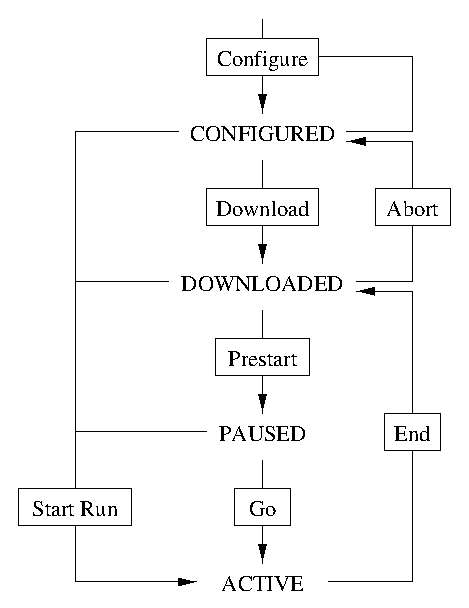
\includegraphics[height=8cm]{daq_trig/coda_scheme.eps}}
     \caption{State Diagram for the DAQ System, controlled by the  Run Control GUI} 
     \label{fig:coda_states}
   \end{center}
\end{figure}

To start a data taking run, click the {\bf\fbox{Prestart}} button.  After a few
seconds a {\bf\fbox{Go}} button should appear.  Click this button.

After {\bf\fbox{Go}} is pressed, a ``Run Info'' form will
pop up.  This form should be updated to reflect the running conditions of
the run about to be started.  The form is filled with default values, but
may be overwritten with the values from the last run by clicking on the
{\bf\fbox{Last Run}} button.  The current values may also be save as default
values if several runs with similar conditions are expected.  When the
{\bf\fbox{OK}} button is clicked, the values held in the form will be written 
to the data file and the run will be started.

Please write sensible comments in the ``Comments'' field.  The first line of 
the
comments will appear in the title of the electronic log book entry made for the
run, so it should be reasonable descriptive.

To modify the layout of this form, edit the file
\verb|~/$DAQROOT/coda2/runparms.default|, consulting an expert if necessary.

To pause/resume a run, use the {\bf\fbox{Pause}}/{\bf\fbox{Go}} buttons on
the pause GUI. 

A run will end if either you click the \fbox{End} button or the event
limit or the data limit (whichever is first) is reached. Event and
data limit can be specified in the \verb|Run Control| GUI. Enter a
number in the appropropriate field and hit $<$return$>$.  Our CODA
system has been configured to allow runs with sizes greater than
2GByte in size. This is done by automatically closing the data file
and opening a new file. Thus a long run will be split into several
segments. The run filenames have the form e93038\_XXXXX.log.N, where N
is the segment number, starting with 0.



\subsubsection{What To Do When Disk Space Runs Out}

\label{disk}
\verb|cdaqs1| has several (As of December 1998, there are 4)
disk partitions of 18 GB each.  The usage of
disk space can be monitored with the ``diskwatch'' screen which is started
from the pop-up menu (middle mouse button on background window).

This windows shows the amount of disk space free on the current disk.
If the free space is 1\% or less, the \fbox{Change Disk}  button should be
pressed.  ``diskwatch'' will then display an empty disk which should be
confirmed with the ``OK'' button.

The data on these partitions is backed up to the mass storage silo
automatically.  Data is deleted from the Hall C data disks manually.
Steve Wood will normally take care of deleting data from the disks, but users
may delete data that has been backed up to the silo with the following
procedure.

Type

\begin{verbatim}
	partition_check N
\end{verbatim}

where N is the number of next partition that you want to use for data taking.
(For example, if data is currently being written to \verb|/cdaqs1/data4|, the 
next
partition to be used will be \verb|/cdaqs1/data1| and thus the command
\verb|partition_check 1| should be issued.

If there are data files on the disk and it is safe to delete them, a prompt 
will appear asking all the files on the partition should be deleted.  
It is safe to
type yes.  At this point all the data files on that partition will be deleted
so anyone trying to replay those runs will need to request them from the silo.

If \verb|partition_check| does not give the option to delete the files, and no
data has been written to the partition for more than 12 hours, please contact
Steve Wood.

To check that the automatic backup is working, do \verb|ls $STAGE| from %$
time to time to see if it contains recent runs.  The STAGE directory is where
runs get queued up to be written to tape.

% HERE Trouble shooting
\section{Trouble Shooting Procedures}
\label{trouble}
When coda crashes usually one of the ROCs or one of the processes got sick and
has to be restarted. The error messages are not always clear. It is 
recommended to try to execute the desired transition again before you start 
rebooting frontends. Often just the connection to the database got lost, which 
can be easily recovered (see below).
If a transition gets stuck because a component failed, it usually takes some 
time until \verb|Run Control| reports back that e.g. {\em Download failed}.
You can try to stop a transition with the \fbox{Cancel} button in the 
\verb|Run Control| GUI. After transition failure and after reboots you 
should always click the \fbox{Reset} button in the \verb|Run Control| GUI and 
configure the run type again, before you start downloading again.   

\begin{itemize}

\item {\bf The connection to the database got lost.}\\
Occurs usually during ``download'' or ``prestart''.
Typical error message: {\em Failed to connect to msqld on cdaqs1}\\
Click \fbox{Reset} in the Run Control GUI and then exit the 
\verb|Run Control| GUI and restart it again. Press the 
\fbox{Connect} button and procede with \fbox{Configure} and 
\fbox{Download}.

\item {\bf Power Outage in the Hall/ sfihms problem}
If Hall C looses power, sfihms (ROC2) (down in the HMS hut) usually looses 
its memory 
and has to be reprogrammed. Detailled description is found in section 
\ref{sfihms}.  

\item {\bf A ROC died}\\
Reboot the particular CPU:  See section \ref{rebooting} for information on
rebooting ROCs.

\item {\bf EB or ER died}\\
Kill EB {\bf and} ER with {\em Ctrl-C} and restart.
To check if they are alive go to the particular 
window and hit a few times $<$return$>$. The prompts
{\em cdaq::ER1$>$} and {\em cdaq::EB1$>$} should appear. You can also use the 
\fbox{Get Status} in the \verb|CODA MASTER| to check the status.

\item {\bf Download Failure} A possible reason for a fail during download
is the following:
Due to repeated downloads the memory of 
the CPUs gets fragmentated and in particular for the older boards with 
smaller memory it can happen that the allocation of the event buffers 
fails. 
If logged into the CPU one would see a message of the type:\\
{\em daLogMsg: partIncr: Cannot malloc a single memory Block for 
data bufs ...}\\ 
In this case one has to do a hardware reboot of the CPU.
Try to \fbox{Cancel} and \fbox{Reset} the transition and proceed with 
\fbox{Configure} after the CPU is rebooted.

\item{\bf Prestart Failure} If Prestart fails some of the components 
might already have prestarted, i.e. they are in the {\em paused} state.
If after eventual reboot, \fbox{Cancel} and \fbox{Reset}, 
i.e. before you try to 
\fbox{Configure} again, some of the components (including EB 
and ER) should still be in {\em paused} state, you have to 
reset them by clicking \fbox{Exit} in the \verb|CODA MASTER| for the 
particular component. After the status of all componenets is either 
{\em booted}, {\em configured} or {\em downloaded} you can proceed with 
\fbox{Configure}.

\item{\bf End Failure} Similarly to the Prestart Failure a fail during End 
can leave components in a state {\em ending}. Exit the ROCs as
described for Prestart Failure. 
Most End Failures make the Event Builder and/or 
Event Recorder unhappy. It's always a good idea to kill and restart 
these two processes after an End Failure.

\item{\bf DD system} The DD system is the memory where the 
Event Builder writes to and the Event Recorder reads from. After a crash 
it is always a good idea to clean the DD system from possible contamination.
In an ``xterm'' type the command \verb|dd_cleanup|. 

\item {\bf No trigger rate at beginning of run or trigger rate goes to 0 
during run}\\
First thing to do is to check the state of the Trigger Supervisor: Click 
\fbox{CHECK} in the \verb|CODA MASTER| and then \fbox{State} in the 
window that pops up. This displays the current state of the TS. If 
\verb|TS Go| and \verb|TS TRIGGER| are enabled and \verb|TS Busy| is 0
then the DAQ is waiting for triggers. 
The two most popular reasons for the absence of triggers are: 
HMS HV down (check the HMS HV display) and prescale 
factors set too high (Check the flag file: \verb|~/\$DAQROOT/coda2/gen.flags|).
Less likely is a hardware failure of one of the components in the electronics
(e.g. the 8LM). In any case this is not a DAQ problem.\\
A \verb|TS Busy| equal to 1 indicates that the TS is not accepting 
triggers anymore which is a DAQ problem.\\
The easiest 
thing to do in this case is to kill all processes (Use the \fbox{KILL ALL} 
button in the \verb|CODA MASTER|)  and reboot all ROCs 
(hardware reboot recommended, see section \ref{rebooting}). However people 
experienced problems with this radical strategy. The advanced idiot 
might try to recover the system in a more controlled way as described in the
following.\\

If the Trigger Supervisor (TS) does not accept triggers anymore, this can 
have two reasons:\\
1. The buffers of the ROCs are full and are not flushed by the 
Event Builder. This indicates an EB or ER problem. The ROCs are most likely 
still ok.\\
2. One of the ROCs died and the TS doesn't receive the Acknowledge from 
this ROC anymore.\\
To see which of the two cases has occured use again the ``ROC and Trigger 
Supervisor Checkout'' window (if not up, click \fbox{CHECK} in the 
\verb|CODA MASTER|). Check the Buffer Status of all ROCs by clicking the 
approriate button. A listing of the allocated memory appears. In the third 
line (column 2 to 4) the number of total (allocated), free and busy (used) 
buffers in the event pool is displayed. If in one of the ROCs the number
of free buffers should be 0, then it's most likely an EB or ER problem.\\
If this is not the case, it is most likely one of the ROCs which has a 
problem. If you hit the button \fbox{State} to get the TS state the Branch
Status is displayed and at least on one branch the \verb|Strobe| and 
\verb|ACK| should be one, indicating that the sick ROC is on this branch. 
Unfortunately the TS does not provide the information which ROC it is.
Use the \fbox{Get Status} button in the \verb|CODA MASTER| or login
to the ROCs as described in section \ref{login} to find out which ROCs 
have a problem.\\

In any case you can still try to \fbox{End} the run, which most probably
will not work properly. You might have to kill Run Control and start it up
again. Even if you use the \fbox{KILL ALL} button in the \verb|CODA MASTER|
(which is probably the appropriate thing to do in this case) you might still
have the problem that some of the ROCs will stay in the state {\em active}). 
In this case you have to exit them with the \fbox{Reset} buttons in the
\verb|CODA MASTER|. If all the componenets are in the state {\em booted},
{\em configured} or {\em downloaded} you can proceed with \fbox{Configure}
and \fbox{Download}

\item {\bf Something that is alive is not necessarily not sick.}  If it is not
clear if all the coda components are working or not, or if you get confused 
about which components need to be restarted, all the components on the Sun 
can be killed with the \fbox{KILL ALL} button in \verb|CODA MASTER| which 
is equivalent to executing the command:
\begin{verbatim}
		~/$DAQROOT/coda2/scripts/coda_cleanup
\end{verbatim}
\end{itemize}


\subsubsection{Remotely Rebooting Crashed or Corrupt VME CPUs}

\label{rebooting}
A software reboot can be done with the \fbox{Reboot} buttons in the 
\verb|CODA MASTER|. This does not always work. Sometimes it's necessary to do 
a hardware reboot. In very rare cases it is necessary to power cycle the 
crates.   
Hardware reboot of all the readout controllers can be done from the 
counting house. See Table \ref{tab:CODA_resets} for reset button locations. The
CPU's located in the counting house are rebooted by pressing the RESET
button on their front panels.  CPU's located in the hall can be reset 
using the {\tt rebootpanel} application which runs on {\tt cdaqs1}.
\begin{center}
\begin{table}[hbt]
\begin{tabular}{|l|c|l|l|}\hline
CPU    & ROC \# & CPU Location               & Reboot button location \\ \hline
sfich1 & 1      & Counting House CH03B07,4-18 & {\it sfich1}          \\
sfich2 & 3      & Counting House CH03B05,4-15 & {\it sfich2}          \\
sfich3 &        &                             & {\it sfich3}          \\
sfisos & 4      & SOS shack                   & {\it sfisos}          \\
sfihms & 2      & HMS hut                     & {\it sfihms}          \\
vmec3  & 20     & Counting House CH03B06      & {\it vmec3}           \\
vmec5  & 5      & Counting House CH03B04      & {\it vmec5}           \\
vmec8  & 8      & Counting House CH03B13      & {\it vmec8}           \\
vmec9  & 9      & Counting House CH03B21      & {\it vmec9}           \\
\hline
\end{tabular}
\begin{tabular}{|l|}
Items in {\it italics} refer to buttons on the {\tt rebootpanel} GUI.\\
\hline
\end{tabular}
\caption{CODA Read Out Controllers reboot button locations\label{tab:CODA_resets}}
\end{table}
\end{center}
It might take a while for the CPU's to reboot.  (The Fastbus
CPU's are the slowest)
The cmlog window will show a message when a particular ROC has rebooted.

\subsection{ROC Login} \label{login}  
To see if a ROC is alive you can connect to the particular CPU
by using the middle mouse button and selecting the CPU you want,
or by {\tt telnet}'ing through the appropriate terminal server
port. See Table~\ref{tab:hctsvx} for a list of port assignments.
For example, to connect to ROC4, type
\begin{verbatim}
        telnet hctsv4 2007
\end{verbatim}
A window will pop up and you will
be logged in. The prompt \verb|->| indicates that you are on the vxworks 
shell.
Type \verb|i| and hit $<$return$>$ to get a listing of the running tasks.
The last item of this list should have the Name {\em ROC} and the Status
{\em Ready} or {\em Pend}. If it does not exist or its status is 
{\em Suspended}, you have to reboot the CPU.\\
You can change to the ROC shell by typing \verb|exit| and 
hitting $<$return$>$ twice. A ROC specific prompt should appear, e.g. 
\verb|cdaq::ROC1>| for sfich1. If this prompt does not appear the ROC 
is sick and the CPU has to be rebooted most likely. With \verb|ctrl-c| 
you can switch back to the vxworks shell. On the ROC shell a set of commands
is available. As an example you can get the status of ROC1 by typing 
\verb|ROC1 status|. This is identical to clicking the button 
\fbox{Get Status} in the \verb|CODA MASTER| but more reliable.     
Be careful when you are logged into the CPU. Misstyped commands can 
hang up everything.  
To logout use \verb|ctrl-]|. At the telnet prompt type \verb|q|.
Generally it's a good idea to keep a window for each ROC open all the times. 
In case of problems the displayed messages might be helpful. 

\subsection{Reprogramming sfihms}
\label{sfihms}
If HALL C looses power ROC 2 might have lost its memory. Already a short power
glitch could cause this. A symptom is that the CPU doesn't reboot anymore.
Reloading the memory can be done from upstairs with the following 
procedure:\\

\noindent
Use an ``xterm'' to login to the terminal server with \verb|telnet LATSRV|.
Username is \verb|cdaq| and Password is \verb|cntrlme|.
Access then the CPU with \verb|set host/lat hcc2|. Password is \verb|vx4daq|.
Hit \verb|<return>| and at the {\em [VXWorks Boot:]} prompt type \verb|c|
to change boot parameters. 
The following list displayes the correct boot parameters for ROC2:\\

\begin{verbatim}
boot device          : dc 
processor number     : 0 
host name            : cdaqs1 
file name            : ~/KERNELS/vx2306_DECFD 
inet on ethernet (e) : 129.57.168.183:fffffc00 
inet on backplane (b): 
host inet (h)        : 129.57.168.15
gateway inet (g)     : 
user (u)             : cdaq 
ftp password (pw) (blank = use rsh): 
flags (f)            : 0x20 
target name (tn)     : sfihms 
startup script (s)   : ~/$DAQROOT/coda2/boot/sfihms.boot 
other (o)            : 
\end{verbatim}

The parameters are listed one by one. Each time you 
hit return the next one is listed until you are back on 
the {\em [VXWorks Boot:]} prompt. For each parameter that is wrong
type in the correct one. Don't try to delete 
wrong parameters just type from there where the cursor is. If you misstype 
don't try to correct just hit return and when you are finished with the list 
start again. When you are done, go through the list again and check all 
entries.
Back at the {\em [VXWorks Boot:]} prompt type \verb|@|
which boots the CPU.\\ 
Use \verb|ctrl-\| to exit and then \verb|lo| to logout from the terminal 
server. 

\subsection{Rebooting other stuff}
There are also a number of CPU's running EPICS and other controls
software.  If controls for High
Voltage or Magnets are not functioning, they may need to be rebooted.
Table \ref{tab:EPICS_resets} gives the location and function of several 
CPU reboot buttons not already listed in Table \ref{tab:CODA_resets}.
Many of these resets are accessed by running the application
{\tt rebootpanel} from an X-session logged in to cdaqs1 (user cdaq).
\begin{center}
\begin{table} [hbt]
%\begin{tabular}{|l|l|l|l|}\hline
\begin{tabular}{|p{1.8in}|p{0.8in}|p{1.5in}|p{1.1in}|}\hline
Function             & CPU    & CPU Location            & Reboot \\ 
                     &        &                         & Button \\\hline
HMS Cryo \& Rotation & vmec2  & HMS Hut                 & {\it vmec2}     \\
SOS HV               & vmec6  & CH03B13,1-11            & {\it vmec6}     \\
M\o ller Cryo,Tgt,Sol  & vmec10 & Near Power Supplies     & {\it vmec10} \dag   \\
M\o ller Quads         & vmec11 & Near Power Supplies     & {\it vmec11} ***\\
Beam Curr, EPICS Rptr& vmec15 & CH03B12-left            & {\it vmec15}    \\
HMS Hall Probes Read & vmec18 & HMS Shield House        & {\it vmec18}    \\
SOS mag controls     & vmec19 & Near Power Supplies     & {\it vmec19}    \\
HMS HV               & vmec20 & CH03B13,1-1             & {\it vmec20}    \\
Slit Box Controls    &        & Pivot Racks             & {\it slitbox}   \\    
Solid Tgt. Rotator   &        & Behind Green Wall       & {\it STGTROT}   \\    
Solid Tgt. Lifter    &        & Behind Green Wall       & {\it STGTLif}   \\  
M\o ller Coll \& Tgt   &        & Behind Green Wall       & {\it MolCol}    \\   
HMS Dipole PS Comm.  & Eldatic& HMS Shield House        & {\it PDS}       \\
HMS Dipole PS Contr. & Dipole & HMS Shield House        & {\it Eldatic}   \\
HMS Q1 Controls      & HMS Q1 & HMS Shield House        & {\it HMSQ1}     \\
HMS Q2 Controls      & HMS Q2 & HMS Shield House        & {\it HMSQ2}     \\
HMS Q3 Controls      & HMS Q3 & HMS Shield House        & {\it HMSQ3}     \\
Fast Raster IOC      & IOCHLC2& HC01Z07                 & {\it IOCHLC2} * **  \\
\hline
\end{tabular}
\begin{tabular}{p{5.5in}}
Items in {\it italics} refer to buttons on the {\tt rebootpanel} GUI.\\
\dag If you reboot VMEC10 (iochc10) you must then RESTORE the Moller cryo saved
parameters. Use the popup menu given by the small blue box on the bottom center
of the M\o ller cryo overview page. Do a "iochc10:NORMAL RESTORE" and keep
hitting ENTER when the popup dialog screen prompts you.\\

* May also be reset from MCC using a software reset.\\

** This reset generates an FSD! Contact MCC first.\\

*** Do not reboot vmec11 (iochc11) unless requested by MCC.\\
\end{tabular}
\caption{EPICS IOC and Device reboot button locations\label{tab:EPICS_resets}}
\end{table}
\end{center}

A reset switch has been moved up to the counting house for the HMS carriage
rotation. One should use this button if the rotation GUI shows interlocks. If
the interlock is real, then the reset button will not clear the interlock. One
needs to press and hold the button for at least 1 to 2 seconds to clear the
Sumito motor controllers. The reset button is located next to the rotation kill
button, on the left section of the counting room console.

\subsection{Online Data Replay}

The Hall~C online data replay is run by a
software package termed the Hall~C engine.
Figure~\ref{fig:7.8} is a flow chart of the Hall~C engine software in which

%hcftest
\begin{figure}
\includegraphics[height=7.5in,width=6in]{daq_trig/engine_flowchart.eps}
\caption{Hall~C Software Engine}
\label{fig:7.8}
\end{figure}

the important codes are named and organized.
Figure~\ref{fig:7.9} is an enhanced view of the HMS event reconstruction section

%hcftest
\begin{figure}
\includegraphics[height=7.5in,width=6in]{daq_trig/recons_flowchart.eps}
%\vspace{8.0in}
\caption{HMS Event Reconstruction Software Engine\label{fig:7.9} }
\end{figure}

of Figure~\ref{fig:7.8} which also lists the functions performed by the codes.
These flow charts and other useful documents, diagrams, and
figures may be found in
\begin{verbatim} ~cdaq/documents. \end{verbatim}

Of particular interest is a document entitled \begin{verbatim}
how_to_replay.txt \end{verbatim}
which
is a step by step outline for a new user describing how to replay runs.
This document may be found in
\begin{verbatim} ~cdaq/documents/analysis_code. \end{verbatim}

